\documentclass[11pt]{article}
\usepackage[a4paper,margin=2.2cm]{geometry}
\usepackage{amsmath}
\usepackage{graphicx}
\usepackage{booktabs}
\usepackage{xcolor}
\usepackage{enumitem}
\usepackage[colorlinks=true,urlcolor=blue!60!black,linkcolor=black]{hyperref}
\usepackage{tcolorbox}
\usepackage{caption}

\setlength{\parindent}{0pt}
\setlength{\parskip}{6pt}

\newcommand{\code}[1]{\texttt{\small #1}}

\begin{document}

\begin{center}
    {\LARGE\bfseries Lab 7 --- Multiplayer Tic-Tac-Toe}\\[2pt]
    {\large OCSF \& EventBus --- Spring 2025--2026}\\[10pt]
    \begin{tabular}{rl}
        Gal Bareket & 326144300\\
        Itai Aviad  & 214891665\\
    \end{tabular}
\end{center}

\hrule
\vspace{8pt}

\textbf{Repository:}\\
\url{https://github.com/SE-Lab-Itai-Gal/labs} \quad (branch \code{lab7}, folder \code{lab7/tictactoe})

\section*{1.\quad What we built}

A two-player networked \textbf{Tic-Tac-Toe} game built on the \textbf{OCSF}
(Object Client--Server Framework) architecture, with a \textbf{JavaFX} graphical
client and the \textbf{EventBus} (GreenRobot) Publish/Subscribe pattern.

Two players connect to the server. When the second player arrives, the server
\textbf{randomly} assigns the symbols \code{X}/\code{O} and randomly decides who
plays first, then the two players take turns. Every move is validated and
broadcast by the server, so the two boards always stay perfectly in sync.

The project is a Maven multi-module project (mirroring the OCSF mediator example):

\begin{itemize}[leftmargin=1.4em,itemsep=1pt]
    \item \code{entities} --- the shared, serializable protocol: \code{GameMessage} + \code{MessageType}.
    \item \code{server} --- the OCSF server (\code{ocsf/*}), \code{GameServer} (game logic) and \code{App} (entry point).
    \item \code{client} --- the JavaFX app (\code{App}, \code{Main}, \code{board.fxml}), the OCSF client
          (\code{GameClient}), the \code{BoardController} and the \code{GameEvent}.
\end{itemize}

\section*{2.\quad How it works}

\textbf{The server is the single source of truth.} A client never draws a move
on its own --- it asks the server, the server checks that it is that player's
turn and the cell is free, applies the move, and \emph{echoes} the validated
move back to \emph{both} players. This is what guarantees the two GUIs cannot
diverge.

\textbf{Networking and UI are decoupled with EventBus.} The OCSF client
(\code{GameClient}) receives objects from the server and re-publishes them on
the EventBus. The \code{BoardController} is a subscriber
(\code{@Subscribe}) and updates the JavaFX scene on the FX thread
(\code{Platform.runLater}). The controller therefore never touches the socket
directly.

\begin{center}
\fbox{\parbox{0.92\textwidth}{\centering\small
\textbf{click} $\rightarrow$ \code{BoardController.sendToServer(MOVE)} $\rightarrow$
\code{GameClient} $\xrightarrow{\text{TCP}}$ \code{GameServer}
(validate $\to$ update $\to$ check win/draw)\\[4pt]
\code{GameServer} $\xrightarrow{\text{TCP}}$ \code{GameClient} $\rightarrow$
\textbf{EventBus.post} $\rightarrow$ \code{BoardController.@Subscribe} $\rightarrow$
\textbf{board updates}
}}
\end{center}

\paragraph{Message protocol.}
\begin{center}
\begin{tabular}{@{}llp{8.4cm}@{}}
\toprule
\textbf{Dir.} & \textbf{Message} & \textbf{Meaning}\\
\midrule
C $\to$ S & \code{"join"} & I want to play.\\
C $\to$ S & \code{MOVE(cell)} & Place my symbol on \code{cell} (0--8).\\
C $\to$ S & \code{"quit"} & Leaving (sent when the window closes).\\
S $\to$ C & \code{WAITING\_FOR\_OPPONENT} & Connected, waiting for a second player.\\
S $\to$ C & \code{GAME\_START(symbol,turn)} & Game started; you are \code{X}/\code{O}; is it your turn.\\
S $\to$ C & \code{MOVE(symbol,cell,turn)} & A validated move (echoed to both players).\\
S $\to$ C & \code{INVALID\_MOVE(text)} & Move rejected (not your turn / cell taken).\\
S $\to$ C & \code{GAME\_OVER(text)} & \code{You win!} / \code{You lose!} / \code{It's a draw!}\\
S $\to$ C & \code{OPPONENT\_DISCONNECTED} & The other player left.\\
S $\to$ C & \code{GAME\_FULL} & A game is already in progress.\\
\bottomrule
\end{tabular}
\end{center}

\section*{3.\quad How to run}

The two runnable jars are in the repository under \code{lab7/tictactoe/dist/}.
JavaFX 21 needs a Java 17+ runtime. The client jar bundles the JavaFX native
libraries for Linux, Windows and macOS, so the same jar runs on all three.

\textbf{On one computer:}
\begin{verbatim}
# 1) start the server (default port 3000)
java -jar tictactoe-server.jar 3000

# 2) start two clients (two windows)
java -jar tictactoe-client.jar localhost 3000
java -jar tictactoe-client.jar localhost 3000
\end{verbatim}

\textbf{On two different computers:}
\begin{enumerate}[leftmargin=1.6em,itemsep=1pt]
    \item Run the server on one machine and note its IP address (e.g. \code{192.168.1.20}).
          Make sure both machines are on the same network and the port is open in the firewall.
    \item On each computer run a client pointing at the server's IP:
          \code{java -jar tictactoe-client.jar 192.168.1.20 3000}
\end{enumerate}

The server listens on port \code{3000} by default; any port \code{> 1024} can be
passed as the first argument to the server and the second argument to each client.

\section*{4.\quad Screenshots}

Two clients connected to one server. The server randomly gave one player
\code{O} and the other \code{X}, and told exactly one of them that it is their
turn:

\begin{figure}[h]
    \centering
    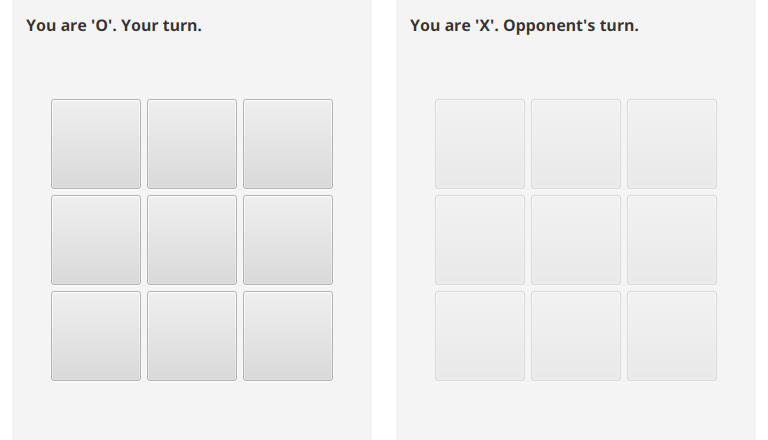
\includegraphics[width=0.85\textwidth]{img/two_clients.png}
    \caption*{\small Two game clients (left: player \code{O}; right: player \code{X}).}
\end{figure}

\textbf{Running on two different computers:}

The server ran on one machine (IP \code{10.100.102.38}); each computer ran a
client connecting to \code{10.100.102.38:3000} over the network. The top
computer won the game (\code{Game over - You win!}) while the bottom one lost
(\code{Game over - You lose!}), showing the same final board on both screens.

\begin{figure}[h]
    \centering
    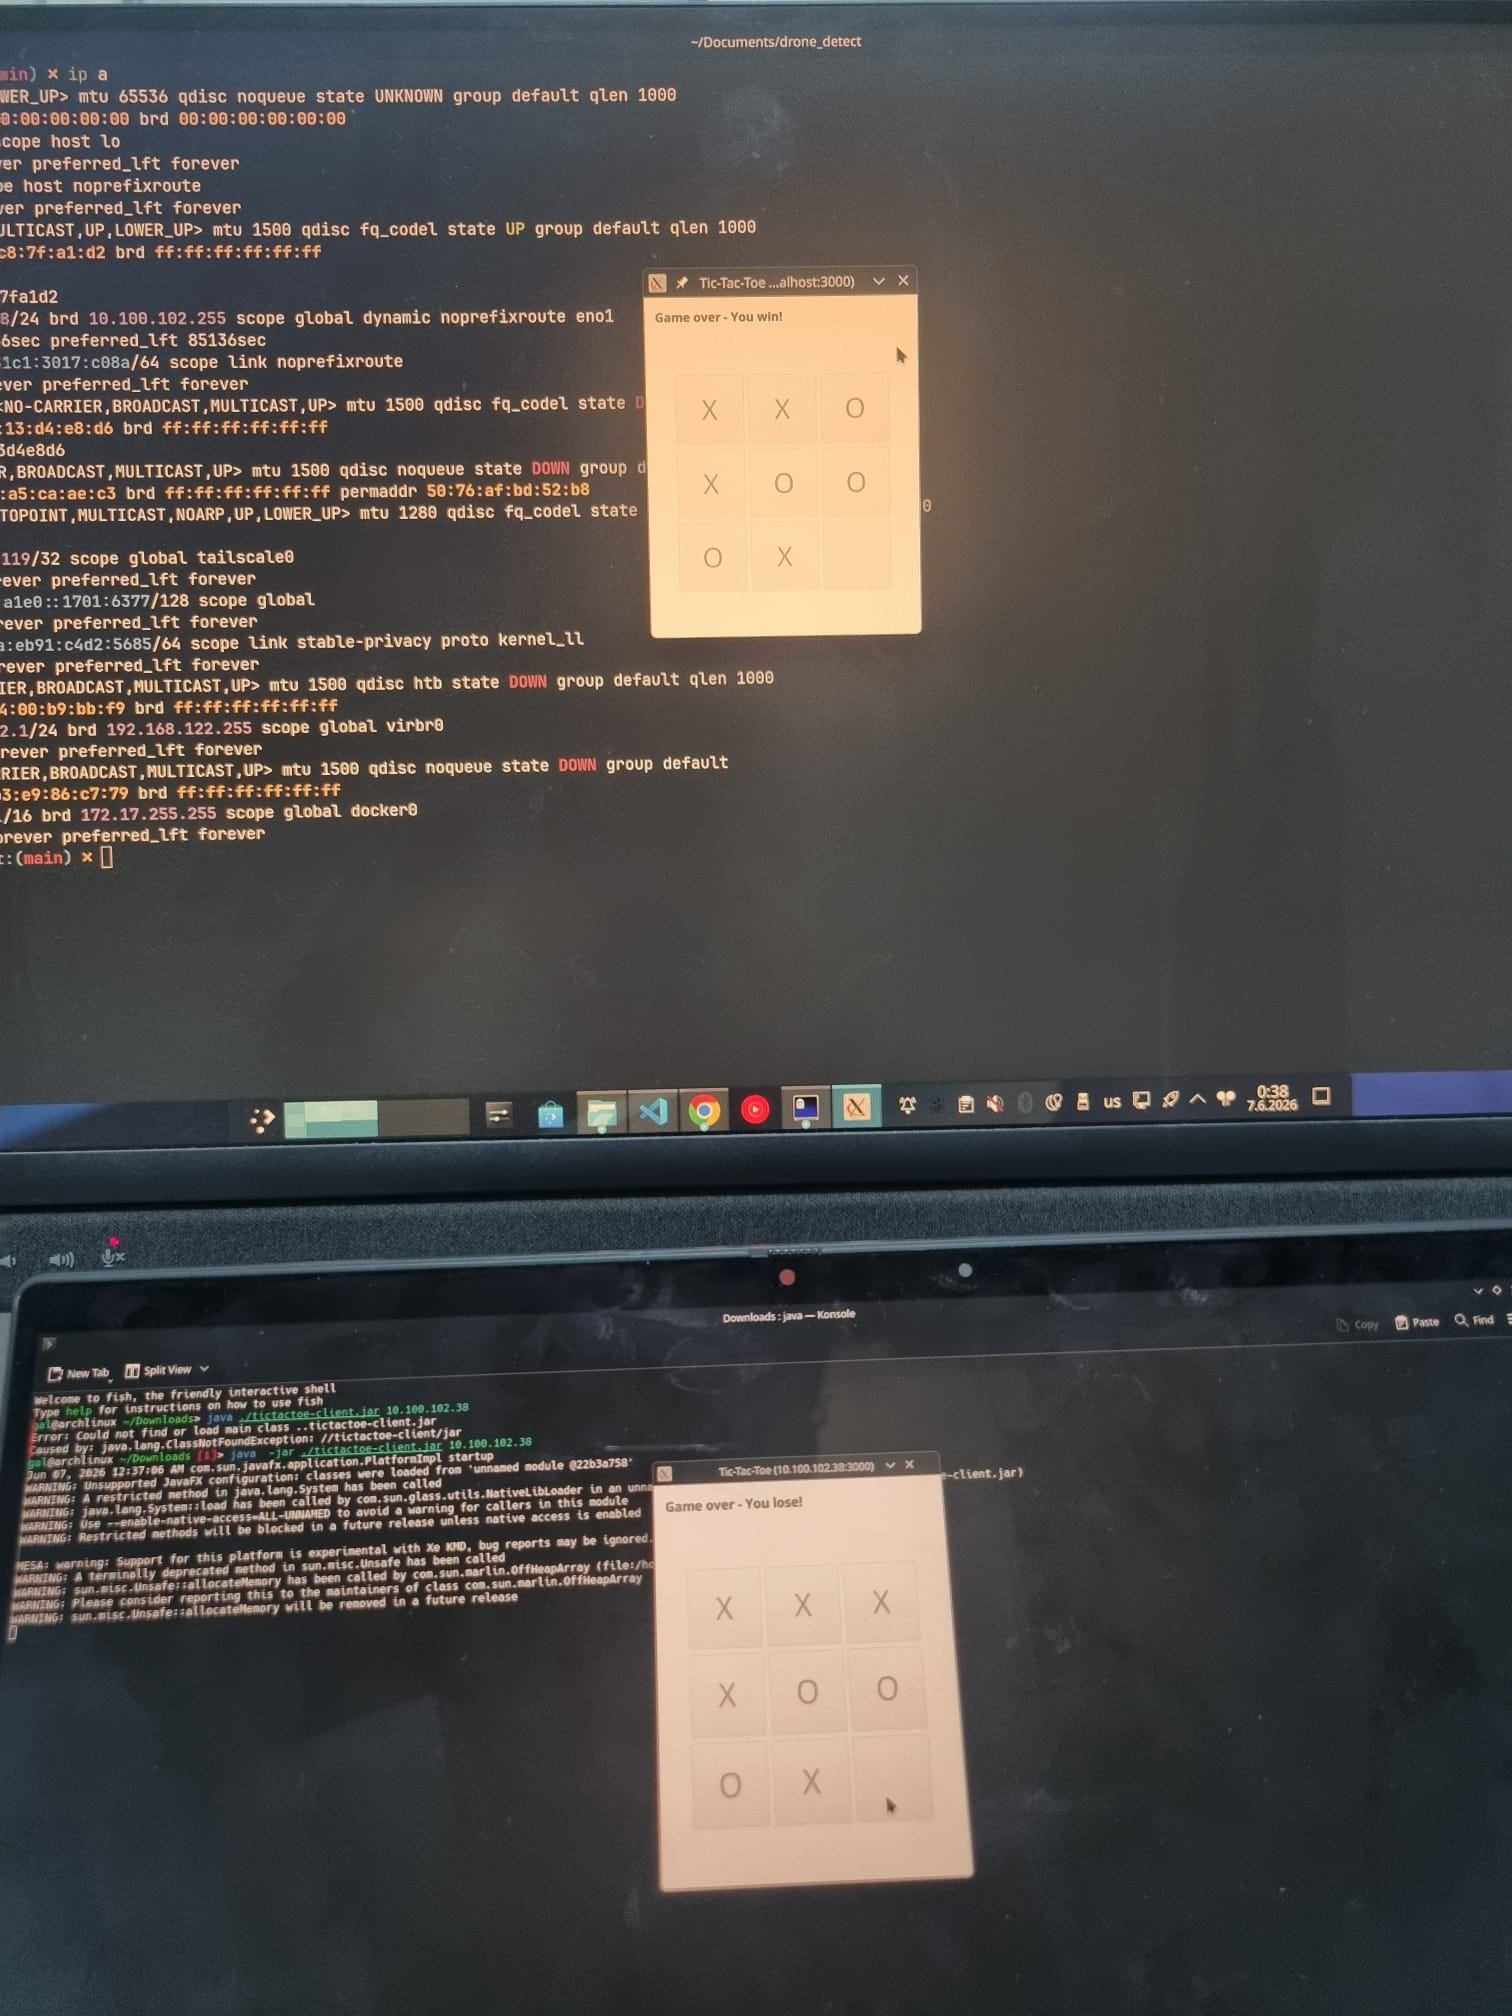
\includegraphics[height=0.78\textheight]{img/two_computers.jpg}
    \caption*{\small The game running on two different computers over the network.}
\end{figure}

\end{document}
